\chapter{The Conical Helix}\label{ch:helix}

\section{The Helix as a Trace on the Cone Surface}

When the original spiral is coupled with the linear height function $z=n$,
a space curve arises that winds along the cone surface. This curve is a
\emph{conical helix}: it combines the radial structure of the spiral with
the vertical structure of the sequence and constitutes the three-dimensional
shape of the construction.

\section{Complete Helix Parametrisation}

\begin{theorem}[Conical Helix]\label{thm:conical-helix}
\begin{equation}
\boxed{
\gamma(\theta) =
\begin{pmatrix}
\frac{6}{\pi^2}\theta \cos(\theta) \\[8pt]
\frac{6}{\pi^2}\theta \sin(\theta) \\[8pt]
-\frac{3}{4} + \frac{3}{\pi}\theta
\end{pmatrix}
}
\end{equation}
\end{theorem}

\begin{figure}[htbp]
  \centering
  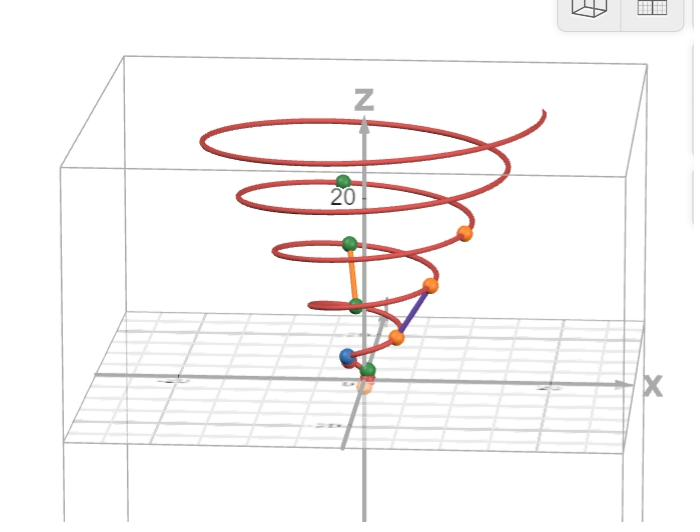
\includegraphics[width=0.75\textwidth]{bilder/Helix_Integer}
  \caption{The conical helix $\gamma(\theta)$ in a perspective view along
    the $z$-axis. The red curve winds upward with increasing radius. The
    green points mark the integer height values $z = n$ with
    $n \equiv 5 \pmod{6}$, and the orange points the values with
    $n \equiv 1 \pmod{6}$. The orange and blue vectors in the lower region
    illustrate the alternating angular spacings
    $\Delta\theta_{\text{major}} = 4\pi/3$ and
    $\Delta\theta_{\text{minor}} = 2\pi/3$ between consecutive integer
    points.}
  \label{fig:helix-integer}
\end{figure}

\section{Derivation of the Velocity and the Arc-Length Integral}

We consider the conical helix
\[
\gamma(t)
= \left(
\frac{6}{\pi^{2}}\,t\cos t,\ 
\frac{6}{\pi^{2}}\,t\sin t,\ 
-\frac{3}{4}+\frac{3}{\pi}\,t
\right),
\]
which consists of a linear height function and a radially growing circular
component. To determine the arc length of this curve, we first require the
speed $\|\gamma'(t)\|$.

\subsection*{1.\ Differentiation of the Components}

We differentiate each component separately. For the first two components we
apply the product rule, since each is a product of $t$ and a trigonometric
function.

\paragraph{First component.}
\[
x(t)=\frac{6}{\pi^{2}}\,t\cos t
\quad\Rightarrow\quad
x'(t)=\frac{6}{\pi^{2}}(\cos t - t\sin t).
\]

\paragraph{Second component.}
\[
y(t)=\frac{6}{\pi^{2}}\,t\sin t
\quad\Rightarrow\quad
y'(t)=\frac{6}{\pi^{2}}(\sin t + t\cos t).
\]

\paragraph{Third component.}
The height function is linear, so:
\[
z(t)=-\frac{3}{4}+\frac{3}{\pi}t
\quad\Rightarrow\quad
z'(t)=\frac{3}{\pi}.
\]

\subsection*{2.\ Speed of the Curve}

The speed is defined as
\[
\|\gamma'(t)\|=\sqrt{x'(t)^2 + y'(t)^2 + z'(t)^2}.
\]

Substituting the derivatives computed above:
\[
\|\gamma'(t)\|^{2}
=
\left(\frac{6}{\pi^{2}}\right)^{2}(\cos t - t\sin t)^{2}
+
\left(\frac{6}{\pi^{2}}\right)^{2}(\sin t + t\cos t)^{2}
+
\left(\frac{3}{\pi}\right)^{2}.
\]

\subsection*{3.\ Simplification of the Trigonometric Expression}

The two squared terms can be simplified by expanding:

\[
(\cos t - t\sin t)^{2}
= \cos^{2}t - 2t\cos t\sin t + t^{2}\sin^{2}t,
\]

\[
(\sin t + t\cos t)^{2}
= \sin^{2}t + 2t\sin t\cos t + t^{2}\cos^{2}t.
\]

Adding both expressions, the mixed terms cancel:
\[
-2t\cos t\sin t + 2t\sin t\cos t = 0.
\]

There remains:
\[
(\cos t - t\sin t)^{2} + (\sin t + t\cos t)^{2}
= \cos^{2}t + \sin^{2}t + t^{2}(\sin^{2}t + \cos^{2}t).
\]

Since $\cos^{2}t + \sin^{2}t = 1$ always holds, we obtain:
\[
(\cos t - t\sin t)^{2} + (\sin t + t\cos t)^{2}
= 1 + t^{2}.
\]

\subsection*{4.\ Final Form of the Speed}

It follows that:
\[
\|\gamma'(t)\|^{2}
= \frac{36}{\pi^{4}}(1+t^{2}) + \frac{9}{\pi^{2}}.
\]

Factoring out $\frac{9}{\pi^4}$ and taking the square root yields the
compact form:

\[
\boxed{
\|\gamma'(t)\|
= \frac{3}{\pi^{2}}\sqrt{4(1+t^{2}) + \pi^{2}}
}.
\]

This representation is particularly well suited for computing the arc length.

\subsection*{5.\ Arc-Length Integral}

The arc length between two parameter values $t_1$ and $t_2$ is therefore:

\[
\boxed{
L(t_{1},t_{2})
= \int_{t_{1}}^{t_{2}}
\frac{3}{\pi^{2}}\sqrt{4(1+t^{2}) + \pi^{2}}\,dt.
}
\]

This integral will be evaluated numerically for specific intervals in what
follows.
%------------
\section{Arc Length of the Helix in the \texorpdfstring{$p$}{p}-Parametrisation}

It is important to emphasise that the formula derived in
Chapter~\ref{sec:bogenlaenge}
\begin{equation}
L_{\mathrm{Spiral}} = \int_{p_1}^{p_2}
\frac{1}{\pi}\sqrt{\frac{3}{p} + \pi^2}\, dp
\end{equation}
computes the arc length of the \emph{two-dimensional spiral} in the
$p$-parametrisation. The arc length of the three-dimensional helix (with the
$\theta$-parametrisation above) is a \emph{different quantity}, since it
includes the additional vertical component $z'(\theta) = 3/\pi$. The
numerical differences between the two arc lengths observed in
Chapter~\ref{ch:examples} arise because they are arc lengths of
\emph{different curves} (the planar spiral on the one hand, the space curve
on the other), not from an error in the parametrisation.

\section{Arc Length Between Integer \texorpdfstring{$n$}{n}-Values}

For integer $n$ we have:
\begin{equation}
\theta(n) = \frac{\pi n}{3} + \frac{\pi}{4}.
\end{equation}

The arc length along the helix is:
\begin{equation}
L = \int_{\theta(n_1)}^{\theta(n_2)}
\sqrt{
\left(\frac{dx}{d\theta}\right)^2
+
\left(\frac{dy}{d\theta}\right)^2
+
\left(\frac{dz}{d\theta}\right)^2
}\, d\theta.
\end{equation}

\section{Example Table}

\begin{table}[ht]
\centering
\caption{Arc lengths between consecutive $n$-values}
\begin{tabular}{ccccc}
\toprule
$n_1 \to n_2$ & $\Delta n$ & Type & $\Delta\theta$ & Arc length \\
\midrule
$1 \to 5$ & 4 & Major & $\frac{4\pi}{3}$ & 11.15519925 \\
$5 \to 7$ & 2 & Minor & $\frac{2\pi}{3}$ & 9.30913741 \\
$7 \to 11$ & 4 & Major & $\frac{4\pi}{3}$ & 26.43477180 \\
\rowcolor{yellow!30}
\textbf{11} $\to$ \textbf{13} & \textbf{2} & \textbf{Minor} & $\frac{2\pi}{3}$ & \textbf{17.16486194} \\
$13 \to 17$ & 4 & Major & $\frac{4\pi}{3}$ & 42.26825081 \\
$17 \to 19$ & 2 & Minor & $\frac{2\pi}{3}$ & 25.11227648 \\
\bottomrule
\end{tabular}
\end{table}

\begin{table}[ht!]
\centering
\caption{Parameter values $\theta_n$, reduced angles, and radii of the
  conical helix. All radii were computed exactly as
  $r_n = (6/\pi^2)\,\theta_n$ and rounded to eight decimal places.}
\begin{tabular}{c c c c c}
\hline
$n$ 
& $\theta_n$ exact 
& $\theta_n$ numerical (rad) 
& Angle mod $360^\circ$ 
& Radius $r_n = \frac{6}{\pi^2}\,\theta_n$ \\
\hline
 5 & $\frac{23\pi}{12}$  & 6.02138592  & $345^\circ$ & 3.66056369 \\
 7 & $\frac{31\pi}{12}$  & 8.11578102  & $105^\circ$ & 4.93380324 \\
11 & $\frac{47\pi}{12}$  & 12.30457123 & $345^\circ$ & 7.48028233 \\
13 & $\frac{55\pi}{12}$  & 14.39896633 & $105^\circ$ & 8.75352187 \\
17 & $\frac{71\pi}{12}$  & 18.58775653 & $345^\circ$ & 11.30000096 \\
19 & $\frac{79\pi}{12}$  & 20.68215164 & $105^\circ$ & 12.57324050 \\
23 & $\frac{95\pi}{12}$  & 24.87094184 & $345^\circ$ & 15.11971959 \\
25 & $\frac{103\pi}{12}$ & 26.96533694 & $105^\circ$ & 16.39295914 \\
29 & $\frac{119\pi}{12}$ & 31.15412715 & $345^\circ$ & 18.93943823 \\
31 & $\frac{127\pi}{12}$ & 33.24852225 & $105^\circ$ & 20.21267777 \\
\hline
\end{tabular}
\end{table}

\section{Full Revolution of the Helix}

A full revolution about the $z$-axis corresponds to $\Delta\theta = 2\pi$.
\begin{equation}
L_{360^\circ}
= \int_{0}^{2\pi}
\sqrt{
\left(\frac{6}{\pi^2}\right)^2(1+\theta^2)
+ \left(\frac{3}{\pi}\right)^2
}\, d\theta
= \boxed{14.5506631745728146863}.
\end{equation}

\subsection{Height Gain per Revolution}

\begin{equation}
\Delta z = \frac{3}{\pi} \cdot 2\pi = 6.
\end{equation}

The helix thus rises by exactly 6 units per revolution.

\section{Geometric Properties of the Helix}

\subsection{Tangent Vector}

\begin{equation}
\gamma'(\theta) =
\begin{pmatrix}
\frac{6}{\pi^2}(\cos\theta - \theta\sin\theta) \\[8pt]
\frac{6}{\pi^2}(\sin\theta + \theta\cos\theta) \\[8pt]
\frac{3}{\pi}
\end{pmatrix}
\end{equation}

\subsection{Curvature}

\begin{remark}[Planar Spiral Curvature as an Approximation]\label{rem:planar-curvature-approx}
The curvature of a space curve $\gamma(t)$ is defined as
$\kappa = |\gamma' \times \gamma''| \, / \, |\gamma'|^3$~\cite{doCarmo1976,Struik1988}
and depends, in the case of the conical helix, on the height component
$z'(\theta) = 3/\pi$. As a tractable approximation one may use the formula
for the planar Archimedean spiral, which for large $\theta$ converges
rapidly to the exact 3D curvature (deviation below $2\,\%$ for $\theta \gtrsim 11$; at $\theta = 2$ it is still $47\,\%$):
\[
  \gamma(\theta) = \bigl(a\theta\cos\theta,\ a\theta\sin\theta,\
  c_0 + c_1\theta\bigr),
  \qquad a = 6/\pi^2, \quad c_1 = 3/\pi,
\]
\end{remark}

\begin{equation}
\kappa(\theta)
= \frac{\theta^2 + 2}{a\,(\theta^2 + 1)^{3/2}},
\qquad
a = \frac{6}{\pi^2}.
\end{equation}

Sample values at the first integer points (each at $\theta = \theta_n$):
\begin{align}
\kappa(\theta_{11}) &= \kappa\!\left(\tfrac{47\pi}{12}\right) \approx 0.134120, \\
\kappa(\theta_{13}) &= \kappa\!\left(\tfrac{55\pi}{12}\right) \approx 0.114512.
\end{align}

The curvature decreases monotonically with increasing $\theta$ --- the helix
becomes progressively straighter along its course.

\begin{theorem}[Exact 3D Curvature and Torsion]\label{thm:3d-curvature-torsion}
For the conical helix

the exact formulae
\begin{align}
\kappa_{\mathrm{3D}}(\theta)
  &= \frac{a\,\sqrt{\,c_1^2\,(\theta^2+4) + a^2\,(\theta^2+2)^2\,}}
          {\bigl(a^2(1+\theta^2) + c_1^2\bigr)^{3/2}},
\label{eq:kappa3d}\\[6pt]
\tau(\theta)
  &= \frac{c_1\,(\theta^2 + 6)}
          {c_1^2\,(\theta^2+4) + a^2\,(\theta^2+2)^2}
\label{eq:torsion}
\end{align}
hold.
\end{theorem}

\begin{proof}
The derivatives of the parametrisation are
\begin{align*}
\gamma'  &= \bigl(a(\cos\theta - \theta\sin\theta),\;
             a(\sin\theta + \theta\cos\theta),\; c_1\bigr),\\
\gamma'' &= \bigl(-a(2\sin\theta + \theta\cos\theta),\;
             a(2\cos\theta - \theta\sin\theta),\; 0\bigr),\\
\gamma'''&= \bigl(a(-3\cos\theta + \theta\sin\theta),\;
             a(-3\sin\theta - \theta\cos\theta),\; 0\bigr).
\end{align*}
By direct computation of the cross product we obtain
\[
  \gamma' \times \gamma''
  = \bigl(-ac_1(2\cos\theta - \theta\sin\theta),\;
          -ac_1(2\sin\theta + \theta\cos\theta),\;
          a^2(\theta^2+2)\bigr)
\]
with $|\gamma' \times \gamma''|^2 = a^2\bigl[c_1^2(\theta^2+4) +
a^2(\theta^2+2)^2\bigr]$ and $|\gamma'|^2 = a^2(1+\theta^2) + c_1^2$.
The curvature follows from $\kappa = |\gamma' \times \gamma''|/|\gamma'|^3$.

For the torsion, the scalar triple product gives
$(\gamma' \times \gamma'') \cdot \gamma''' = a^2 c_1(\theta^2+6)$,
whence $\tau = (\gamma' \times \gamma'') \cdot \gamma''' \,/\,
|\gamma' \times \gamma''|^2$.
\end{proof}

\begin{remark}\label{rem:asymptotic-torsion}
For $\theta \to \infty$ we have asymptotically
\begin{gather*}
  \kappa_{\mathrm{3D}}(\theta) \sim \frac{1}{a\theta} = \frac{1}{r(\theta)},
  \qquad
  \tau(\theta) \sim \frac{c_1}{a^2\theta^2} = \frac{\pi^3}{12\,\theta^2},\\
  \text{i.e.}\quad
  \lim_{\theta\to\infty} \theta^2\,\tau(\theta) = \frac{c_1}{a^2}
  = \frac{\pi^3}{12} = 2.583856\ldots
\end{gather*}
The torsion is positive for every $\theta$ --- in contrast to the
planar spiral, whose torsion vanishes identically --- but decays
quadratically to zero, while the curvature approaches that of a circle
of the current radius $r(\theta)$: locally the helix straightens its
screw component faster than its bending. Numerically,
$\theta^2\tau(\theta) = 2.5692\ldots$ at $\theta = 10$ and
$2.583856\ldots$ at $\theta = 10^4$.

At the integer points $\theta_n = \pi n/3 + \pi/4 = \pi Q/12$ with
$Q = 4n+3$ (Section~\ref{subsec:Q}), the identity $Q^2 = 48k(n)+1$ turns the
asymptotics into an arithmetic statement:
\begin{equation}\label{eq:torsion_Q}
  \tau(\theta_n) \;\approx\; \frac{12\pi}{Q^2}
  \;=\; \frac{12\pi}{48\,k(n)+1},
\end{equation}
with relative error $1.9 \cdot 10^{-4}$ at $n = 47$ and
$4.5 \cdot 10^{-5}$ at $n = 97$. The torsion at a lattice point is thus
asymptotically the reciprocal of the same quantity $48k+1$ whose square
root $Q$ parametrises the construction
(Section~\ref{subsec:Q}); the differential-geometric
screw rate and the arithmetic of the sequence are read off from one
number. Note that $\tau$ is a smooth, monotone function of $\theta$:
it does not distinguish the two residue classes, nor primes from
composites --- that information lies in the occupation of the points,
not in the geometry of the curve.
\end{remark}

\section{Integer Points on the Helix}

Solving $z(\theta_n) = n$:
\begin{align}
-\frac{3}{4} + \frac{3}{\pi}\theta_n &= n, \\
\theta_n &= \frac{\pi}{3}\left(n + \frac{3}{4}\right), \\
\theta_n &= \frac{\pi}{3}n + \frac{\pi}{4}.
\end{align}

Thus all $n \equiv 1,5 \pmod{6}$ occur as discrete points on the helix.

\begin{proposition}[Determination of the height function]\label{prop:height-uniqueness}
Let $z(\theta) = b\theta + c$ be an affine height function. The
requirement of one period per revolution,
$z(\theta + 2\pi) = z(\theta) + 6$, forces $b = 6/(2\pi) = 3/\pi$. The
remaining constant is fixed by the vertex--apex identification
$z(0) = n_0 = -\tfrac34$ of Chapter~\ref{ch:cone}, giving
$c = -\tfrac34$. No further normalisation enters: slope and offset of
the height function are determined by one structural requirement and
one explicit identification, and with these values the integer heights
are attained exactly at $\theta_n = \pi n/3 + \pi/4$.
\end{proposition}
The complete analysis of these integer points --- including the prime number
corollary --- follows in Chapter~\ref{ch:primes}.
